\documentclass[9pt,twocolumn,twoside]{../../styles/osajnl}
\usepackage{fancyvrb}
\journal{i524} 

\title{\LaTeX\ Puppet - Automatic Configration management }

\author[1,*]{Ashok Vuppada}

\affil[1]{School of Informatics and Computing, Bloomington, IN 47408, U.S.A.}

\affil[*]{Corresponding authors: ashokmadhu66@gmail.com}

\dates{project-000, \today}

\ociscodes{Cloud, I524}

% replace this with your url in github/gitlab
\doi{\url{https://github.com/justbbusy/sp17-i524/tree/master/paper2/S17-IO-3024/report.pdf}}


\begin{abstract}

Cloud providers today need to deliver pre installed infrastructure ,
operating system or programing language as per the service level
agreements. There would be need to maintain multiple instances with
various dependencies installed. It would become extremely impossible
to maintain the configurations manually ,hence configuration
management tools become a necessary in the cloud era. Puppet is one of
the configuration management tool available today

{Sharelatex} systems.\newline
\end{abstract}

\setboolean{displaycopyright}{true}

\begin{document}

\maketitle

\section{Introduction}

Puppet can mean the programming language in which the end state
required is defined. unlike the procedural steps there is no need to
know the required steps to achieve the end state , puppet would
internally manage the required steps and ensures the end state is
achieved. The same Puppet language code works between various
operating systems. \cite{www-infoq}

Puppet Language alone cannot achieve the configuration management
required , puppet code needs to be maintained on regular basis to
ensure the required dependencies are properly getting installed on the
client servers. Puppet platform provides the required framework to
maintain the puppet code. \cite{www-infoq}

\section{Architecture}

Catalog is the file which contains the end state of required at the
client , it is defined in puppet language. This file is maintained at
the puppet master, It would be downloaded by puppet client from the
puppet master when it is run. The changes are applied by compiling and
running the catalog.\cite{www-docpuppet}

Puppet agent is a daemon process runs on the client machine where the
configuration is required to be managed. Puppet master is a daemon
process that runs on the host which manages the configuration across
the various clients. The puppet agent and master would be communicated
through a secure SSL connection. The puppet master would keep checking
with client if the required installations are done or not , if there
is any change in the end state required at a given client the puppet
agent would run and ensures the end state is changed as per the
configuration. It is also possible to define the time interval
required for the puppet master to check with the client.\cite{www-slashroot}

Puppet is developed by Puppet Labs using ruby language and released as
GNU General Public License (GPL) until version 2.7.0 and the Apache
License 2.0 after that.\cite{www-wiki-puppet}

\begin{figure}[htbp]
\centering
\fbox{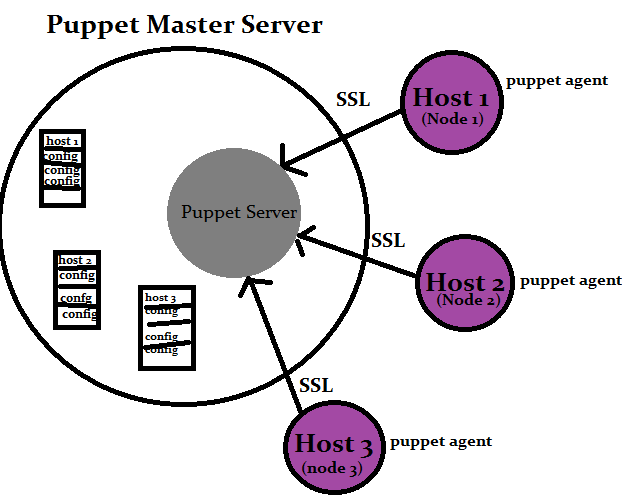
\includegraphics[width=\linewidth]{images/Arch.png}}
\caption{Puppet Master Puppet Client Communication}
\label{fig:Puppet}
\end{figure}


\section{Configuration}


\subsection {Puppet Master Configuration}

\begin{figure}[htbp]
\centering
\fbox{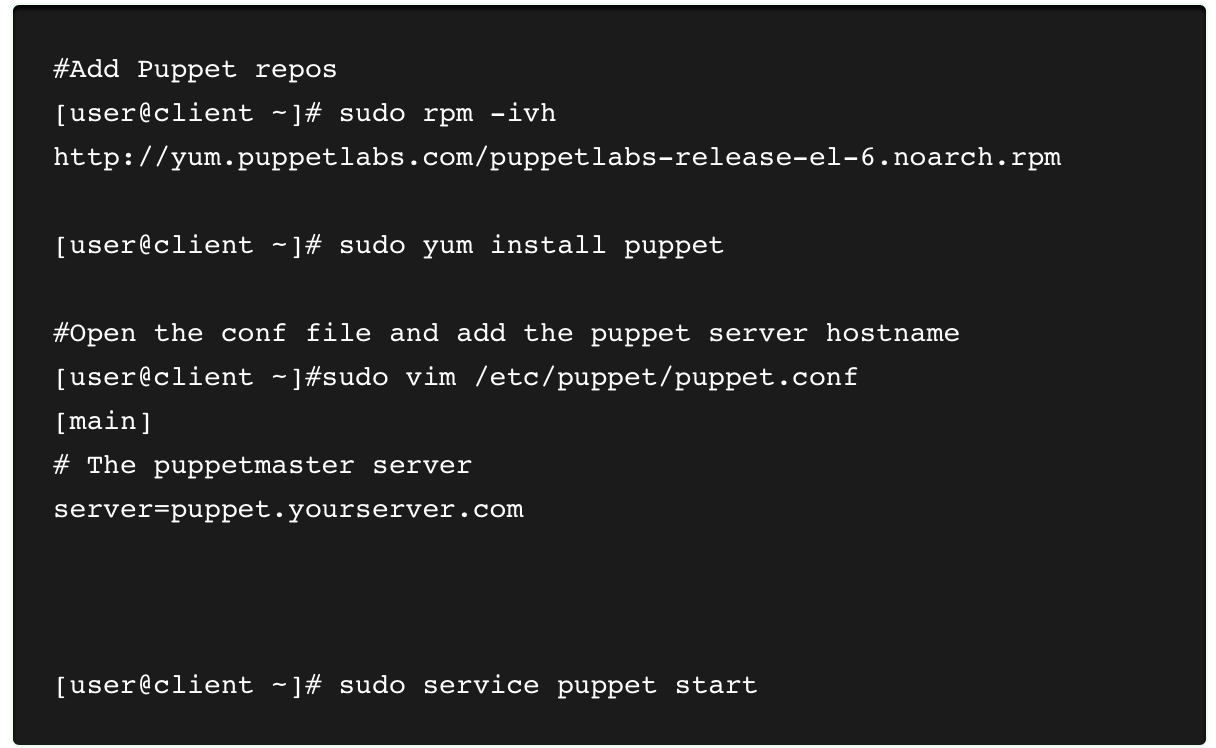
\includegraphics[width=\linewidth]{images/Inst1.png}}
\caption{Puppet Master Configuration}
\label{fig:Puppet}
\end{figure} \cite{www-techarena}


\subsection {Puppet Client Configuration}

\begin{figure}[htbp]
\centering
\fbox{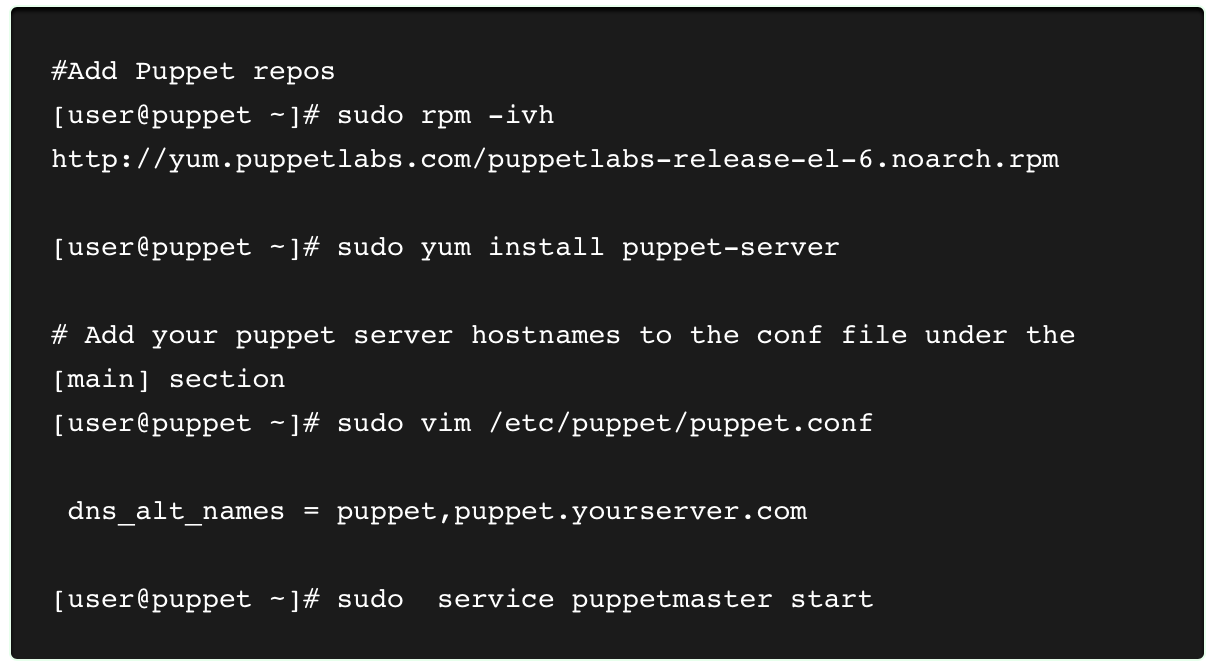
\includegraphics[width=\linewidth]{images/Inst2.png}}
\caption{Puppet Client Configuration}
\label{fig:Puppet}
\end{figure}  \cite{www-techarena}

\subsection { If Client needs to changes immediately}

\begin{figure}[htbp]
\centering
\fbox{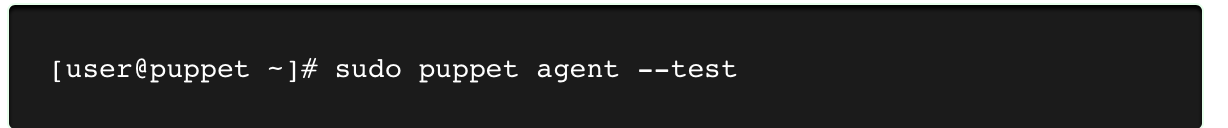
\includegraphics[width=\linewidth]{images/Inst3.png}}
\caption{If Client needs to changes immediately}
\label{fig:Puppet}
\end{figure}  \cite{www-techarena}

\section{Advantages} 

\begin{enumerate}

\item Puppet Labs provides very good support for this tool.
\item Good interface and runs on almost all operating systems.
\item Installation and setup is simple
\item Strong reporting capabilities

\end{enumerate} \cite{www-intigue}


\section{Disadvantages}

\begin{enumerate}

\item For more advanced tasks, one need to use the CLI, which is
Ruby-based makes it necessary to have ruby knowledge.
\item Support for pure-Ruby versions is being scaled back.
\item DSL and a design that does not focus on
simplicity, the Puppet code base can grow large, unwieldy, and hard to
pick up for new people in your organization at higher scale.
\item Model-driven approach means less control compared to code-driven
approaches.\cite{www-intigue} 

\end{enumerate}

\section{Conclusion}

The need of configuration is essential with the cloud offering with
various tools like Chef , Ansible , Puppet , Salt etc in market gives
freedom for the configuration management team to use the the
applicable tool based on the case to case need.



% Bibliography

\bibliography{references}
 

\newpage

\appendix



\end{document}
